\chapter{Business Ecosystem Analysis}

\section{BCD Networking Platform Ecosystem}

The BCD (Business Community Deutschland) platform represents a sophisticated ecosystem designed to facilitate high-value business networking and deal flow generation. At its core, the platform serves as a central hub connecting diverse stakeholder groups through a carefully curated network architecture that emphasizes quality, exclusivity, and mutual value creation.

\subsection{Core Platform Architecture}

The BCD platform operates as a multi-sided marketplace that brings together entrepreneurs, investors, C-level executives, and family offices in a structured environment designed to maximize networking efficiency and deal flow quality. The platform's architecture is built around three fundamental principles: exclusivity, quality curation, and value-driven interactions.

\textbf{Platform Positioning:} BCD positions itself as a premium business networking platform that goes beyond traditional networking by focusing specifically on deal flow generation and high-value business connections. Unlike general networking platforms, BCD emphasizes quality over quantity, ensuring that each member brings significant value to the network.

\textbf{Value Proposition:} The platform's primary value proposition centers on three key pillars: (1) access to high-quality deal flow for investors, (2) strategic networking opportunities for entrepreneurs and executives, and (3) curated introductions that lead to meaningful business relationships and transactions.

\subsection{Member Segments and Value Creation}

\subsubsection{Entrepreneurs and Startup Founders}
The entrepreneur segment represents one of the platform's primary user groups, consisting of growth-stage company founders and CEOs seeking capital, strategic partnerships, and market expansion opportunities. These members typically operate companies with \$1M+ in annual revenue and are actively seeking growth capital or strategic partnerships.

\textbf{Value Delivered:} Entrepreneurs gain access to a curated network of investors, potential strategic partners, and industry experts who can provide not only capital but also strategic guidance, market insights, and business development opportunities.

\textbf{Engagement Model:} The platform facilitates direct connections through structured networking events, one-on-one introductions, and deal flow presentations that allow entrepreneurs to showcase their businesses to qualified investors and potential partners.

\subsubsection{Investors and Venture Capitalists}
The investor segment includes venture capitalists, angel investors, and institutional investors actively seeking quality deal flow and investment opportunities. These members typically manage significant investment portfolios and are looking for growth-stage companies with strong market potential.

\textbf{Value Delivered:} Investors gain access to a pre-screened pipeline of investment opportunities, reducing the time and resources required for deal sourcing and due diligence. The platform's curation process ensures that only qualified opportunities reach the investor network.

\textbf{Engagement Model:} Investors participate in deal flow presentations, networking events, and direct introductions to entrepreneurs, with the platform providing comprehensive due diligence support and deal structuring assistance.

\subsubsection{C-Level Executives}
The C-level executive segment consists of senior executives from established companies seeking strategic partnerships, innovation opportunities, and business development connections. These members typically hold leadership positions in mid to large enterprises with significant market presence.

\textbf{Value Delivered:} Executives gain access to innovative startups, potential acquisition targets, and strategic partnership opportunities that can drive corporate innovation and business growth.

\textbf{Engagement Model:} The platform facilitates strategic introductions, innovation showcases, and partnership development opportunities through structured events and direct networking.

\subsubsection{Family Offices}
The family office segment represents ultra-high-net-worth families seeking investment opportunities, strategic partnerships, and legacy planning solutions. These members typically manage significant family wealth and are looking for long-term investment and partnership opportunities.

\textbf{Value Delivered:} Family offices gain access to curated investment opportunities, strategic partnership possibilities, and legacy planning resources that align with their long-term wealth preservation and growth objectives.

\textbf{Engagement Model:} The platform provides exclusive access to investment opportunities, strategic partnership development, and legacy planning resources through private events and direct introductions.

\subsection{Service Delivery Channels}

\subsubsection{Digital Communication Platform (WhatsApp)}
The platform leverages WhatsApp as a primary communication channel, providing real-time networking opportunities and deal flow updates. This digital-first approach ensures immediate access to network opportunities and facilitates rapid deal flow communication.

\textbf{Implementation:} The WhatsApp integration provides instant messaging capabilities, deal flow alerts, and networking updates, ensuring that members can respond quickly to time-sensitive opportunities.

\subsubsection{Accelerated Networking Program (Fast Track)}
The Fast Track program provides intensive networking opportunities through structured events and direct introductions designed to accelerate relationship building and deal flow generation.

\textbf{Implementation:} The program includes curated networking events, direct introductions, and deal flow presentations that maximize the efficiency of networking interactions and accelerate relationship development.

\subsubsection{Digital Networking Forums}
Digital forums provide ongoing networking opportunities through virtual events, webinars, and online discussions that complement in-person networking activities.

\textbf{Implementation:} The digital forums include regular webinars, virtual networking events, and online discussion groups that facilitate ongoing relationship building and knowledge sharing.

\subsubsection{Traditional Networking Events (Stammtische)}
Traditional networking events, known as "Stammtische," provide in-person networking opportunities through regular gatherings that foster relationship building and community development.

\textbf{Implementation:} These events include regular networking gatherings, industry-specific meetups, and exclusive member events that facilitate face-to-face relationship building and community development.

\subsection{Value Flow Dynamics}

\subsubsection{Deal Flow Generation}
The platform's primary value flow centers on deal flow generation, connecting entrepreneurs with investors through a structured process that ensures quality and relevance.

\textbf{Process:} The deal flow process includes initial screening, due diligence support, and structured presentations that maximize the likelihood of successful connections and transactions.

\subsubsection{Knowledge Exchange}
The platform facilitates knowledge exchange between members, creating a learning environment that benefits all participants through shared insights and best practices.

\textbf{Implementation:} Knowledge exchange occurs through educational events, peer learning opportunities, and structured knowledge sharing sessions that benefit all network participants.

\begin{figure}[h]
\centering
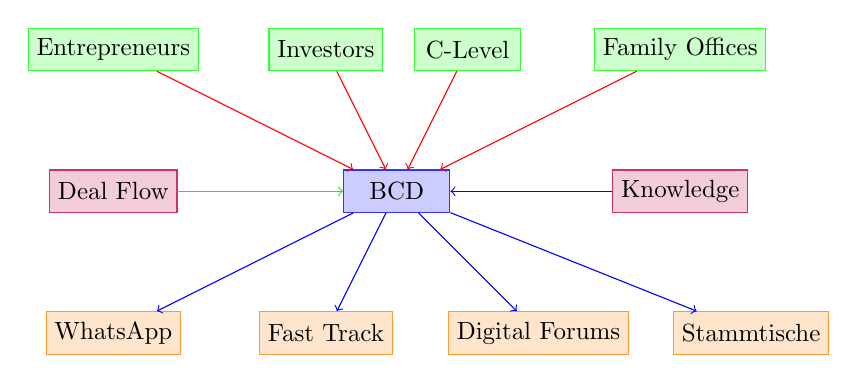
\begin{tikzpicture}[
    scale=0.9,
    transform shape,
    box/.style={rectangle, draw, minimum width=1.5cm, minimum height=0.6cm, align=center},
    platform/.style={box, fill=blue!20, draw=blue!80},
    member/.style={box, fill=green!20, draw=green!80},
    service/.style={box, fill=orange!20, draw=orange!80},
    value/.style={box, fill=purple!20, draw=purple!80},
    arrow/.style={->}
]

% Core Platform
\node[platform] (bcd) at (0,0) {BCD};

% Member Segments
\node[member] (entrepreneurs) at (-4,2) {Entrepreneurs};
\node[member] (investors) at (-1,2) {Investors};
\node[member] (executives) at (1,2) {C-Level};
\node[member] (family) at (4,2) {Family Offices};

% Services
\node[service] (whatsapp) at (-4,-2) {WhatsApp};
\node[service] (retreats) at (-1,-2) {Fast Track};
\node[service] (events) at (2,-2) {Digital Forums};
\node[service] (stammtisch) at (5,-2) {Stammtische};

% Value Flows
\node[value] (deals) at (-4,0) {Deal Flow};
\node[value] (knowledge) at (4,0) {Knowledge};

% Connections
\draw[arrow, red] (entrepreneurs) -- (bcd);
\draw[arrow, red] (investors) -- (bcd);
\draw[arrow, red] (executives) -- (bcd);
\draw[arrow, red] (family) -- (bcd);

\draw[arrow, blue] (bcd) -- (whatsapp);
\draw[arrow, blue] (bcd) -- (retreats);
\draw[arrow, blue] (bcd) -- (events);
\draw[arrow, blue] (bcd) -- (stammtisch);

\draw[arrow, green] (deals) -- (bcd);
\draw[arrow, blue] (knowledge) -- (bcd);

\end{tikzpicture}
\caption{BCD Business Networking Platform Ecosystem}
\label{fig:bcd-platform-ecosystem}
\end{figure}

\section{Competitive Landscape Radar Analysis}

The competitive landscape for business networking platforms is complex and multi-dimensional, with various players occupying distinct market positions based on their focus areas, target audiences, and value propositions. The radar analysis provides a comprehensive view of how BCD positions itself relative to key competitors across six critical dimensions: global reach, digital capabilities, regional focus, deal flow emphasis, exclusivity, and network quality.

\subsection{Competitive Positioning Framework}

The radar analysis framework evaluates competitors across six key dimensions that are critical to success in the business networking space. Each dimension represents a strategic factor that influences platform positioning and competitive advantage.

\textbf{Global Scale (0°):} This dimension measures the geographic reach and international presence of networking platforms. Global scale is critical for platforms seeking to serve multinational businesses and investors with international interests.

\textbf{Digital Innovation (60°):} This dimension assesses the platform's technological capabilities, digital-first approach, and ability to leverage technology for enhanced networking experiences and operational efficiency.

\textbf{Regional Focus (120°):} This dimension evaluates the platform's depth of local market knowledge, regional network strength, and ability to serve specific geographic markets with tailored services and local expertise.

\textbf{Deal Flow Emphasis (180°):} This dimension measures the platform's focus on facilitating business transactions, investment opportunities, and deal flow generation versus general networking and relationship building.

\textbf{Exclusivity (240°):} This dimension assesses the platform's membership criteria, quality standards, and ability to maintain an exclusive, high-value network that attracts premium members.

\textbf{Network Quality (300°):} This dimension evaluates the overall quality of network connections, member caliber, and the platform's ability to facilitate meaningful, high-value business relationships.

\subsection{Competitor Analysis and Positioning}

\subsubsection{YPO (Young Presidents' Organization)}
\textbf{Position:} Global Scale (0°) - High Score (2.5/3)

YPO represents the gold standard in global executive networking, with an unparalleled international presence spanning 142 countries and over 30,000 members. The organization's global scale is its primary competitive advantage, enabling it to serve multinational executives and businesses with international interests.

\textbf{Strengths:}
\begin{itemize}
    \item Unmatched global network with presence in 142 countries
    \item Rigorous membership criteria ensuring high-quality network
    \item Comprehensive international chapter structure
    \item Strong brand recognition and credibility
    \item Extensive global event calendar and networking opportunities
\end{itemize}

\textbf{Market Position:} YPO dominates the global scale dimension, serving as the premier international executive networking platform with unmatched geographic reach and international market penetration.

\subsubsection{EO (Entrepreneurs' Organization)}
\textbf{Position:} Digital Innovation (60°) - High Score (2.0/3)

EO has established itself as a leader in digital innovation within the business networking space, leveraging technology to enhance member experiences and facilitate global connectivity. The organization's digital-first approach enables efficient networking across its global network.

\textbf{Strengths:}
\begin{itemize}
    \item Advanced digital platform and mobile applications
    \item Global virtual networking capabilities
    \item Technology-enabled learning and development programs
    \item Digital-first approach to member engagement
    \item Scalable technology infrastructure
\end{itemize}

\textbf{Market Position:} EO leads in digital innovation, providing a modern, technology-enabled networking experience that appeals to digitally-savvy entrepreneurs and business leaders.

\subsubsection{Vistage}
\textbf{Position:} Regional Focus (120°) - Medium Score (1.5/3)

Vistage demonstrates strong regional focus through its local chapter structure and market-specific services. The organization's regional approach enables deep market knowledge and tailored services for local business communities.

\textbf{Strengths:}
\begin{itemize}
    \item Strong regional chapter structure and local market presence
    \item Market-specific services and programs
    \item Deep local market knowledge and expertise
    \item Regional networking opportunities and events
    \item Local business community integration
\end{itemize}

\textbf{Market Position:} Vistage excels in regional focus, providing deep local market expertise and tailored services that address specific regional business needs and opportunities.

\subsubsection{Chief}
\textbf{Position:} Deal Flow Emphasis (180°) - Low Score (1.2/3)

Chief focuses primarily on women's leadership development and career advancement rather than deal flow generation. The platform emphasizes mentorship, career development, and professional networking over business transactions and investment opportunities.

\textbf{Strengths:}
\begin{itemize}
    \item Specialized focus on women's leadership development
    \item Strong mentorship and career advancement programs
    \item Modern digital-first approach to networking
    \item Comprehensive educational programs and events
    \item Growing market presence in women's leadership space
\end{itemize}

\textbf{Market Position:} Chief occupies a specialized niche in women's leadership development, with limited focus on deal flow generation and business transactions.

\subsubsection{Tiger 21}
\textbf{Position:} Exclusivity (240°) - High Score (1.8/3)

Tiger 21 maintains high exclusivity through rigorous membership criteria and focus on ultra-high-net-worth individuals. The platform's exclusive approach ensures a premium network quality and attracts members with significant wealth and investment capacity.

\textbf{Strengths:}
\begin{itemize}
    \item Rigorous membership criteria ensuring high exclusivity
    \item Focus on ultra-high-net-worth individuals
    \item Premium network quality and member caliber
    \item Exclusive access to high-value investment opportunities
    \item Strong emphasis on wealth preservation and investment
\end{itemize}

\textbf{Market Position:} Tiger 21 excels in exclusivity, maintaining a premium network of ultra-high-net-worth individuals with significant investment capacity and wealth management needs.

\subsubsection{BCD Platform}
\textbf{Position:} Network Quality (300°) - High Score (2.3/3)

BCD positions itself as a high-quality networking platform with strong emphasis on network quality and deal flow generation. The platform's curated approach ensures meaningful connections and high-value business relationships.

\textbf{Strengths:}
\begin{itemize}
    \item Curated membership ensuring high network quality
    \item Strong focus on deal flow generation and business transactions
    \item Regional expertise in DACH market
    \item Digital-first approach with modern technology platform
    \item Strategic partnerships with ecosystem players
\end{itemize}

\textbf{Market Position:} BCD excels in network quality, providing a curated, high-value network focused on deal flow generation and meaningful business relationships.

\subsection{Strategic Implications and Market Opportunities}

\subsubsection{Competitive Advantages}
Based on the radar analysis, BCD's primary competitive advantages include:
\begin{itemize}
    \item \textbf{Network Quality Focus:} Strong emphasis on curated, high-quality network connections
    \item \textbf{Deal Flow Specialization:} Specialized focus on deal flow generation and business transactions
    \item \textbf{Regional Expertise:} Deep DACH market knowledge and local network strength
    \item \textbf{Digital Innovation:} Modern technology platform with digital-first approach
    \item \textbf{Strategic Positioning:} Unique position bridging traditional networking and investment platforms
\end{itemize}

\subsubsection{Market Opportunities}
The competitive analysis reveals several market opportunities:
\begin{itemize}
    \item \textbf{Regional Gap:} Opportunity to dominate DACH region with specialized services
    \item \textbf{Deal Flow Focus:} Growing demand for platforms specializing in deal flow generation
    \item \textbf{Digital Transformation:} Shift towards digital-first networking approaches
    \item \textbf{Ecosystem Integration:} Opportunity to integrate with broader startup and investment ecosystems
    \item \textbf{Quality Differentiation:} Market demand for high-quality, curated networking experiences
\end{itemize}

\subsubsection{Strategic Recommendations}
Based on the competitive analysis, BCD should focus on:
\begin{itemize}
    \item \textbf{Regional Leadership:} Establish dominant position in DACH region with specialized services
    \item \textbf{Deal Flow Excellence:} Develop superior deal flow generation capabilities and processes
    \item \textbf{Digital Innovation:} Continue investment in technology platform and digital capabilities
    \item \textbf{Quality Curation:} Maintain high standards for network quality and member curation
    \item \textbf{Ecosystem Partnerships:} Develop strategic partnerships with accelerators, incubators, and service providers
\end{itemize}

\begin{figure}[h]
\centering
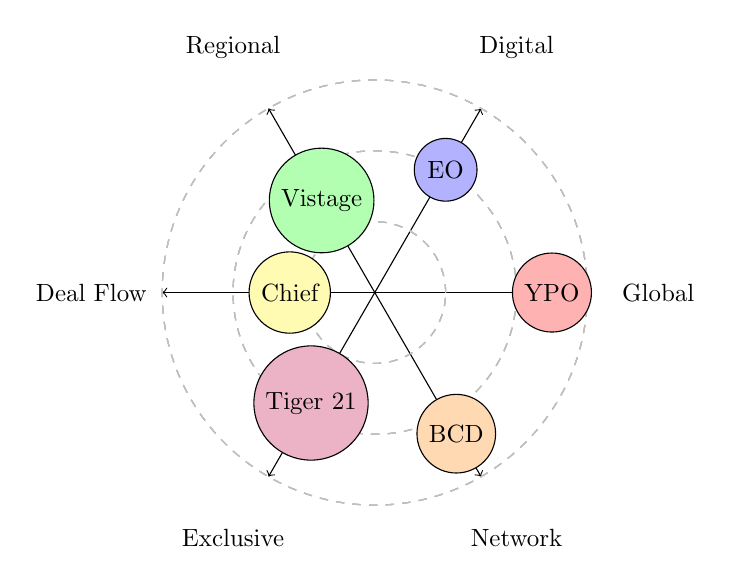
\begin{tikzpicture}[
    scale=0.9,
    transform shape,
    radar/.style={circle, draw, minimum size=0.8cm, align=center},
    axis/.style={->},
    grid/.style={dashed, gray!50}
]

% Radar grid - simplified
\foreach \angle in {0, 60, 120, 180, 240, 300} {
    \draw[axis] (0,0) -- (\angle:3);
    \draw[grid] (0,0) circle (1);
    \draw[grid] (0,0) circle (2);
    \draw[grid] (0,0) circle (3);
}

% Competitor positions
\node[radar, fill=red!30] at (0:2.5) {YPO};
\node[radar, fill=blue!30] at (60:2.0) {EO};
\node[radar, fill=green!30] at (120:1.5) {Vistage};
\node[radar, fill=yellow!30] at (180:1.2) {Chief};
\node[radar, fill=purple!30] at (240:1.8) {Tiger 21};
\node[radar, fill=orange!30] at (300:2.3) {BCD};

% Axis labels
\node at (0:4) {Global};
\node at (60:4) {Digital};
\node at (120:4) {Regional};
\node at (180:4) {Deal Flow};
\node at (240:4) {Exclusive};
\node at (300:4) {Network};

\end{tikzpicture}
\caption{Competitive Landscape Radar Analysis}
\label{fig:competitive-radar}
\end{figure}

\section{Comprehensive Competitor Analysis}

\subsection{Direct Competitors: Traditional Networking Platforms}

\subsubsection{YPO (Young Presidents' Organization)}
\textbf{Profile:} Founded in 1950, YPO is the world's premier leadership organization for chief executives, with over 30,000 members across 142 countries. The organization focuses on peer learning and idea exchange among business leaders.

\textbf{Key Strengths:}
\begin{itemize}
    \item Global network spanning 142 countries with 30,000+ members
    \item Exclusive membership criteria (CEO/President under 45, \$10M+ company revenue)
    \item Established brand recognition and credibility in executive circles
    \item Comprehensive learning programs and peer-to-peer education
    \item Strong regional chapter structure with local networking events
\end{itemize}

\textbf{Competitive Advantages:}
\begin{itemize}
    \item 70+ years of market presence and established trust
    \item Rigorous membership screening ensuring high-quality network
    \item International scale with local market penetration
    \item Comprehensive educational and leadership development programs
    \item Strong alumni network and lifetime membership benefits
\end{itemize}

\textbf{Market Position:} Premium global executive network with focus on leadership development and peer learning.

\textbf{Threat Level:} High - Established market leader with significant resources and brand recognition.

\subsubsection{EO (Entrepreneurs' Organization)}
\textbf{Profile:} Founded in 1987, EO is a global network of entrepreneurs with over 15,000 members across 61 countries. The organization focuses on peer-to-peer learning and business growth support.

\textbf{Key Strengths:}
\begin{itemize}
    \item Entrepreneur-focused membership with 15,000+ members globally
    \item Forum-based peer learning methodology
    \item Strong emphasis on business growth and scaling
    \item Regional chapter structure with local networking
    \item Comprehensive educational programs and events
\end{itemize}

\textbf{Competitive Advantages:}
\begin{itemize}
    \item Specialized focus on entrepreneurs and business scaling
    \item Proven forum methodology for peer learning
    \item Global network with local market expertise
    \item Strong emphasis on business growth outcomes
    \item Comprehensive event calendar and educational resources
\end{itemize}

\textbf{Market Position:} Entrepreneur-focused networking platform with emphasis on business growth and scaling.

\textbf{Threat Level:} Medium-High - Direct competitor in entrepreneur networking space.

\subsubsection{Vistage}
\textbf{Profile:} Founded in 1957, Vistage is a CEO coaching and peer advisory organization with over 45,000 members worldwide, focusing on executive leadership development and business performance.

\textbf{Key Strengths:}
\begin{itemize}
    \item 45,000+ members across 20 countries
    \item CEO coaching and peer advisory focus
    \item Proven methodology for business performance improvement
    \item Strong emphasis on leadership development
    \item Comprehensive educational programs and resources
\end{itemize}

\textbf{Competitive Advantages:}
\begin{itemize}
    \item Specialized focus on CEO coaching and peer advisory
    \item Proven methodology for business performance improvement
    \item Strong emphasis on leadership development and coaching
    \item Comprehensive educational programs and resources
    \item Established track record of member business growth
\end{itemize}

\textbf{Market Position:} CEO coaching and peer advisory platform with focus on leadership development.

\textbf{Threat Level:} Medium - Differentiated focus on coaching and advisory services.

\subsubsection{Chief}
\textbf{Profile:} Founded in 2019, Chief is a private network designed for women in leadership positions, with over 20,000 members across the United States and United Kingdom.

\textbf{Key Strengths:}
\begin{itemize}
    \item 20,000+ women leaders across US and UK
    \item Focus on women's leadership development
    \item Modern digital-first approach to networking
    \item Strong emphasis on mentorship and career advancement
    \item Comprehensive educational programs and events
\end{itemize}

\textbf{Competitive Advantages:}
\begin{itemize}
    \item Specialized focus on women's leadership development
    \item Modern digital-first approach to networking
    \item Strong emphasis on mentorship and career advancement
    \item Comprehensive educational programs and events
    \item Growing market presence in women's leadership space
\end{itemize}

\textbf{Market Position:} Women-focused leadership network with modern digital approach.

\textbf{Threat Level:} Medium - Specialized focus on women's leadership development.

\subsubsection{Tiger 21}
\textbf{Profile:} Founded in 1999, Tiger 21 is a peer-to-peer learning network for high-net-worth individuals, with over 1,000 members managing \$75 billion in assets.

\textbf{Key Strengths:}
\begin{itemize}
    \item 1,000+ high-net-worth members managing \$75B+ assets
    \item Focus on wealth preservation and investment strategies
    \item Peer-to-peer learning methodology
    \item Strong emphasis on investment education
    \item Exclusive membership criteria and screening
\end{itemize}

\textbf{Competitive Advantages:}
\begin{itemize}
    \item Specialized focus on high-net-worth individuals
    \item Strong emphasis on wealth preservation and investment
    \item Peer-to-peer learning methodology
    \item Exclusive membership criteria ensuring quality network
    \item Proven track record in investment education
\end{itemize}

\textbf{Market Position:} High-net-worth investment and wealth management network.

\textbf{Threat Level:} Medium - Specialized focus on wealth management and investment.

\section{Stakeholder Ecosystem Constellation}

\begin{figure}[h]
\centering
\begin{tikzpicture}[
    scale=1.0,
    transform shape,
    core/.style={circle, draw, fill=blue!30, minimum size=0.5cm},
    primary/.style={circle, draw, fill=green!30, minimum size=0.4cm},
    secondary/.style={rectangle, draw, fill=orange!30, minimum size=0.4cm},
    tertiary/.style={diamond, draw, fill=purple!30, minimum size=0.4cm},
    arrow/.style={->}
]

% Central BCD Platform
\node[core] (bcd) at (0,0) {BCD};

% Primary Stakeholders (closest to core)
\node[primary] (entrepreneurs) at (-2,1.5) {Ent};
\node[primary] (investors) at (2,1.5) {Inv};
\node[primary] (executives) at (-2,-1.5) {C-Level};
\node[primary] (family) at (2,-1.5) {Family};

% Secondary Stakeholders
\node[secondary] (accelerators) at (-3.5,0) {Accel};
\node[secondary] (banks) at (3.5,0) {Banks};
\node[secondary] (vc) at (0,2.5) {VCs};
\node[secondary] (angels) at (0,-2.5) {Angels};

% Tertiary Stakeholders
\node[tertiary] (legal) at (-5,0.9) {Legal};
\node[tertiary] (accounting) at (-5,-0.9) {Acct};
\node[tertiary] (marketing) at (5,0.9) {Mktg};
\node[tertiary] (tech) at (5,-0.9) {Tech};

% Core connections
\draw[arrow] (bcd) -- (entrepreneurs);
\draw[arrow] (bcd) -- (investors);
\draw[arrow] (bcd) -- (executives);
\draw[arrow] (bcd) -- (family);

% Primary to secondary
\draw[arrow] (entrepreneurs) -- (accelerators);
\draw[arrow] (investors) -- (banks);
\draw[arrow] (executives) -- (vc);
\draw[arrow] (family) -- (angels);

% Secondary to tertiary
\draw[arrow] (accelerators) -- (legal);
\draw[arrow] (accelerators) -- (accounting);
\draw[arrow] (banks) -- (marketing);
\draw[arrow] (banks) -- (tech);

% Value flows
\draw[arrow, red] (entrepreneurs) -- (investors);
\draw[arrow, blue] (executives) -- (family);

\end{tikzpicture}
\caption{Stakeholder Ecosystem Constellation}
\label{fig:stakeholder-constellation}
\end{figure}

\subsection{Cross-Sectional Analysis: Incubator and Accelerator Ecosystems}

\subsubsection{Y Combinator}
\textbf{Profile:} Founded in 2005, Y Combinator is one of the world's most successful startup accelerators, having funded over 3,000 companies with a combined valuation of over \$300 billion.

\textbf{Partnership Opportunities:}
\begin{itemize}
    \item Potential collaboration on startup ecosystem development
    \item Cross-referral opportunities for growth-stage companies
    \item Joint educational programs and events
    \item Shared resources for startup scaling and investment
    \item Network expansion opportunities for both organizations
\end{itemize}

\textbf{Competitive Dynamics:}
\begin{itemize}
    \item Different focus areas (accelerator vs. networking platform)
    \item Complementary services and value propositions
    \item Potential for strategic partnerships and collaborations
    \item Shared target audience of entrepreneurs and investors
    \item Opportunities for cross-ecosystem value creation
\end{itemize}

\subsubsection{Techstars}
\textbf{Profile:} Founded in 2006, Techstars is a global startup accelerator with over 2,700 companies in its portfolio and operations in 150+ cities worldwide.

\textbf{Partnership Opportunities:}
\begin{itemize}
    \item Global network expansion opportunities
    \item Joint educational programs and events
    \item Cross-referral opportunities for startups and investors
    \item Shared resources for startup ecosystem development
    \item Collaborative programs for growth-stage companies
\end{itemize}

\textbf{Competitive Dynamics:}
\begin{itemize}
    \item Different service offerings (acceleration vs. networking)
    \item Complementary value propositions and target audiences
    \item Potential for strategic partnerships and collaborations
    \item Shared focus on entrepreneur and investor networks
    \item Opportunities for ecosystem-wide value creation
\end{itemize}

\subsubsection{Station F}
\textbf{Profile:} Founded in 2017, Station F is the world's largest startup campus, housing over 1,000 startups and providing comprehensive support services for early-stage companies.

\textbf{Partnership Opportunities:}
\begin{itemize}
    \item European market expansion opportunities
    \item Joint programs for startup ecosystem development
    \item Cross-referral opportunities for European startups
    \item Shared resources for startup support and scaling
    \item Collaborative events and educational programs
\end{itemize}

\textbf{Competitive Dynamics:}
\begin{itemize}
    \item Different focus areas (campus vs. networking platform)
    \item Complementary services and value propositions
    \item Potential for strategic partnerships and collaborations
    \item Shared target audience of entrepreneurs and investors
    \item Opportunities for European ecosystem development
\end{itemize}

\subsubsection{Rocket Internet}
\textbf{Profile:} Founded in 2007, Rocket Internet is a global venture builder and startup incubator, having built and invested in over 200 companies across various industries.

\textbf{Partnership Opportunities:}
\begin{itemize}
    \item Global venture building and investment opportunities
    \item Cross-referral opportunities for startups and investors
    \item Joint programs for startup ecosystem development
    \item Shared resources for venture building and scaling
    \item Collaborative events and educational programs
\end{itemize}

\textbf{Competitive Dynamics:}
\begin{itemize}
    \item Different focus areas (venture building vs. networking)
    \item Complementary services and value propositions
    \item Potential for strategic partnerships and collaborations
    \item Shared target audience of entrepreneurs and investors
    \item Opportunities for global ecosystem development
\end{itemize}

\section{Regulatory Compliance Framework}

\begin{figure}[h]
\centering
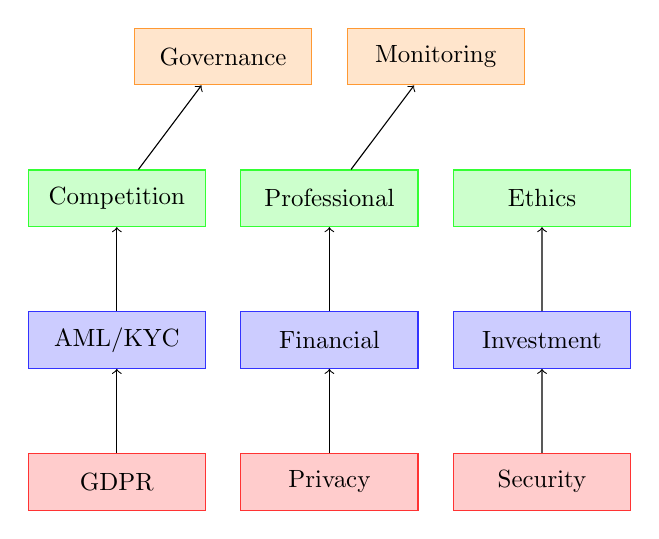
\begin{tikzpicture}[
    scale=0.9,
    transform shape,
    layer/.style={rectangle, draw, minimum width=2.5cm, minimum height=0.8cm, align=center},
    foundation/.style={layer, fill=red!20, draw=red!80},
    core/.style={layer, fill=blue!20, draw=blue!80},
    operational/.style={layer, fill=green!20, draw=green!80},
    strategic/.style={layer, fill=orange!20, draw=orange!80},
    arrow/.style={->}
]

% Regulatory layers
\node[foundation] (gdpr) at (0,0) {GDPR};
\node[foundation] (privacy) at (3,0) {Privacy};
\node[foundation] (security) at (6,0) {Security};

\node[core] (aml) at (0,2) {AML/KYC};
\node[core] (financial) at (3,2) {Financial};
\node[core] (investment) at (6,2) {Investment};

\node[operational] (competition) at (0,4) {Competition};
\node[operational] (professional) at (3,4) {Professional};
\node[operational] (ethics) at (6,4) {Ethics};

\node[strategic] (governance) at (1.5,6) {Governance};
\node[strategic] (monitoring) at (4.5,6) {Monitoring};

% Connections
\draw[arrow] (gdpr) -- (aml);
\draw[arrow] (privacy) -- (financial);
\draw[arrow] (security) -- (investment);

\draw[arrow] (aml) -- (competition);
\draw[arrow] (financial) -- (professional);
\draw[arrow] (investment) -- (ethics);

\draw[arrow] (competition) -- (governance);
\draw[arrow] (professional) -- (monitoring);

\end{tikzpicture}
\caption{Regulatory Compliance Framework}
\label{fig:regulatory-framework}
\end{figure}

\subsection{Emerging Digital-First Networks}

\subsubsection{LinkedIn Premium}
\textbf{Profile:} LinkedIn's premium networking features provide digital-first networking opportunities for professionals across various industries and career stages.

\textbf{Competitive Advantages:}
\begin{itemize}
    \item Massive user base with global reach
    \item Advanced networking and communication tools
    \item Comprehensive professional profiles and recommendations
    \item Integrated job search and career development features
    \item Strong emphasis on professional networking and career advancement
\end{itemize}

\textbf{Market Position:} Digital-first professional networking platform with global reach.

\textbf{Threat Level:} Medium - Different focus on professional networking vs. business networking.

\subsubsection{Digital-First Platforms}
\textbf{Profile:} Various digital-first networking platforms are emerging, offering specialized networking services for specific industries and professional groups.

\textbf{Competitive Advantages:}
\begin{itemize}
    \item Digital-first approach to networking
    \item Specialized focus on specific industries and professional groups
    \item Advanced technology and user experience
    \item Scalable business models and global reach
    \item Strong emphasis on user engagement and community building
\end{itemize}

\textbf{Market Position:} Digital-first networking platforms with specialized focus areas.

\textbf{Threat Level:} Medium - Emerging competition in digital networking space.

\section{Value Flow Network Analysis}

The Value Flow Network Analysis provides a mathematical framework for understanding how value circulates through the BCD platform ecosystem. This analysis employs concepts from fluid dynamics and graph theory to model the complex interactions between different network components and identify optimal flow patterns for value creation and distribution.

\subsection{Fluid Dynamics Model of Value Flow}

The platform's value flow can be modeled using fluid dynamics principles, where value acts as a fluid moving through a network of interconnected channels. This mathematical approach provides insights into flow efficiency, bottlenecks, and optimization opportunities.

\subsubsection{Continuity Equation for Value Conservation}

The fundamental principle of value conservation in the network can be expressed through the continuity equation:

\begin{equation}
\frac{\partial \rho}{\partial t} + \nabla \cdot (\rho \mathbf{v}) = S
\end{equation}

Where:
\begin{itemize}
    \item $\rho$ represents the density of value at any point in the network
    \item $\mathbf{v}$ is the velocity vector of value flow
    \item $S$ represents sources and sinks of value in the network
    \item $\nabla \cdot$ is the divergence operator
\end{itemize}

This equation ensures that value is neither created nor destroyed within the network, but rather redistributed through various channels and processes.

\subsubsection{Navier-Stokes Equations for Value Flow Dynamics}

The complex dynamics of value flow can be modeled using modified Navier-Stokes equations:

\begin{equation}
\rho \left(\frac{\partial \mathbf{v}}{\partial t} + (\mathbf{v} \cdot \nabla)\mathbf{v}\right) = -\nabla p + \mu \nabla^2 \mathbf{v} + \mathbf{f}
\end{equation}

Where:
\begin{itemize}
    \item $\rho$ is the value density
    \item $\mathbf{v}$ is the value flow velocity
    \item $p$ represents the pressure gradient driving value flow
    \item $\mu$ is the viscosity coefficient representing friction in value transfer
    \item $\mathbf{f}$ represents external forces affecting value flow
\end{itemize}

In the context of the BCD platform, the pressure gradient ($\nabla p$) represents the difference in value potential between different network nodes, driving value flow from high-potential to low-potential areas.

\subsection{Graph Theory Analysis of Network Structure}

The platform's network structure can be analyzed using graph theory, providing insights into connectivity patterns, centrality measures, and network resilience.

\subsubsection{Network Representation as a Directed Graph}

The BCD platform can be represented as a directed graph $G = (V, E)$, where:
\begin{itemize}
    \item $V$ is the set of vertices representing network nodes (entrepreneurs, investors, executives, family offices)
    \item $E$ is the set of directed edges representing value flow connections
    \item Each edge $(u, v) \in E$ has a weight $w(u, v)$ representing the strength of the value flow
\end{itemize}

\subsubsection{Centrality Measures for Network Analysis}

Several centrality measures provide insights into the network's structure and dynamics:

\textbf{Degree Centrality:}
\begin{equation}
C_D(v) = \frac{\text{deg}(v)}{|V| - 1}
\end{equation}

This measures the number of connections for each node, identifying highly connected members who serve as network hubs.

\textbf{Betweenness Centrality:}
\begin{equation}
C_B(v) = \sum_{s \neq v \neq t} \frac{\sigma_{st}(v)}{\sigma_{st}}
\end{equation}

Where $\sigma_{st}$ is the number of shortest paths between nodes $s$ and $t$, and $\sigma_{st}(v)$ is the number of those paths that pass through node $v$. This identifies nodes that act as bridges between different network segments.

\textbf{Eigenvector Centrality:}
\begin{equation}
C_E(v) = \frac{1}{\lambda} \sum_{u \in N(v)} C_E(u)
\end{equation}

This measures the influence of a node based on the centrality of its neighbors, identifying influential members who are connected to other influential members.

\subsection{Value Flow Optimization Using Network Flow Theory}

The platform's value flow can be optimized using network flow theory, which provides mathematical tools for maximizing value transfer while respecting capacity constraints.

\subsubsection{Maximum Flow Problem}

The value flow optimization can be formulated as a maximum flow problem:

\begin{equation}
\text{Maximize: } \sum_{v \in V} f(s, v)
\end{equation}

Subject to:
\begin{align}
f(u, v) &\leq c(u, v) \quad \text{(Capacity constraints)} \\
\sum_{u \in V} f(u, v) &= \sum_{w \in V} f(v, w) \quad \text{(Flow conservation)} \\
f(u, v) &\geq 0 \quad \text{(Non-negative flow)}
\end{align}

Where:
\begin{itemize}
    \item $f(u, v)$ is the flow from node $u$ to node $v$
    \item $c(u, v)$ is the capacity of the connection from $u$ to $v$
    \item $s$ is the source node representing value generation
\end{itemize}

\subsubsection{Minimum Cost Flow Problem}

For more sophisticated optimization, we can formulate a minimum cost flow problem:

\begin{equation}
\text{Minimize: } \sum_{(u,v) \in E} c(u,v) \cdot f(u,v)
\end{equation}

Subject to flow conservation and capacity constraints, where $c(u,v)$ represents the cost of transferring value through the connection $(u,v)$.

\subsection{Barrier Analysis Using Potential Theory}

The barriers to value flow can be analyzed using potential theory, where barriers create potential differences that impede flow.

\subsubsection{Potential Barrier Model}

The effect of barriers on value flow can be modeled as:

\begin{equation}
\phi(x) = \phi_0 + \sum_{i} \frac{q_i}{4\pi \epsilon |x - x_i|}
\end{equation}

Where:
\begin{itemize}
    \item $\phi(x)$ is the potential at point $x$
    \item $\phi_0$ is the baseline potential
    \item $q_i$ represents the strength of barrier $i$
    \item $x_i$ is the location of barrier $i$
    \item $\epsilon$ is the permeability of the network medium
\end{itemize}

\subsection{Network Resilience and Robustness Analysis}

The platform's resilience to disruptions can be analyzed using graph theory concepts.

\subsubsection{Connectivity Analysis}

The network's connectivity can be measured using:

\textbf{Algebraic Connectivity:}
\begin{equation}
\lambda_2 = \min_{x \perp \mathbf{1}} \frac{x^T L x}{x^T x}
\end{equation}

Where $L$ is the Laplacian matrix of the graph. Higher values indicate greater network connectivity and resilience.

\textbf{Network Diameter:}
\begin{equation}
D = \max_{u,v \in V} d(u,v)
\end{equation}

Where $d(u,v)$ is the shortest path distance between nodes $u$ and $v$. Smaller diameters indicate more efficient value flow.

\subsection{Mathematical Optimization of Platform Performance}

The platform's performance can be optimized using mathematical programming techniques.

\subsubsection{Multi-Objective Optimization}

The platform optimization can be formulated as:

\begin{equation}
\text{Maximize: } \alpha \cdot \text{Value Flow} + \beta \cdot \text{Network Quality} + \gamma \cdot \text{User Satisfaction}
\end{equation}

Subject to:
\begin{align}
\text{Capacity Constraints: } & \sum_{v \in N(u)} f(u,v) \leq C_u \\
\text{Quality Constraints: } & Q(u,v) \geq Q_{\min} \\
\text{Trust Constraints: } & T(u,v) \geq T_{\min}
\end{align}

Where $\alpha$, $\beta$, and $\gamma$ are weighting factors for different objectives.

\subsection{Practical Applications and Implementation}

The mathematical framework provides practical tools for platform optimization:

\subsubsection{Flow Rate Optimization}
\begin{itemize}
    \item \textbf{Deal Flow Matching:} Optimize matching algorithms to maximize successful connections
    \item \textbf{Knowledge Transfer:} Design efficient knowledge sharing mechanisms
    \item \textbf{Capital Flow:} Optimize investment flow from investors to entrepreneurs
\end{itemize}

\subsubsection{Barrier Reduction Strategies}
\begin{itemize}
    \item \textbf{Trust Building:} Implement verification systems and reputation mechanisms
    \item \textbf{Privacy Protection:} Develop secure data handling protocols
    \item \textbf{Quality Assurance:} Establish rigorous curation and validation processes
\end{itemize}

\subsubsection{Network Growth Optimization}
\begin{itemize}
    \item \textbf{Strategic Recruitment:} Target high-centrality potential members
    \item \textbf{Connection Optimization:} Facilitate connections that maximize network value
    \item \textbf{Resilience Building:} Create redundant pathways for value flow
\end{itemize}

This mathematical framework provides a rigorous foundation for understanding and optimizing the BCD platform's value flow dynamics, enabling data-driven decisions for platform development and growth.

\begin{figure}[h]
\centering
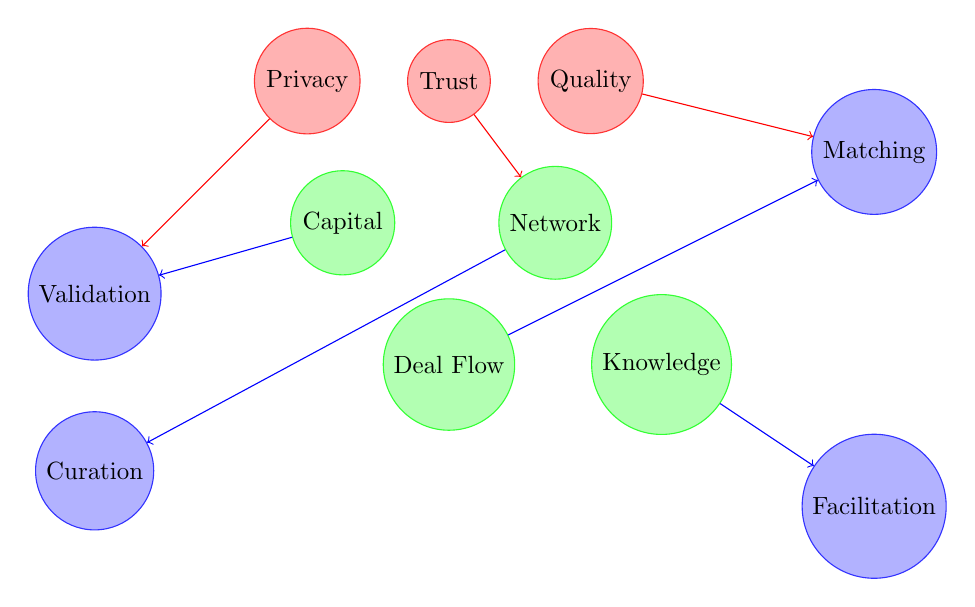
\begin{tikzpicture}[
    scale=0.9,
    transform shape,
    node/.style={circle, draw, minimum size=0.8cm, align=center},
    value/.style={node, fill=green!30, draw=green!80},
    flow/.style={node, fill=blue!30, draw=blue!80},
    barrier/.style={node, fill=red!30, draw=red!80},
    arrow/.style={->}
]

% Value nodes
\node[value] (deals) at (0,0) {Deal Flow};
\node[value] (knowledge) at (3,0) {Knowledge};
\node[value] (network) at (1.5,2) {Network};
\node[value] (capital) at (-1.5,2) {Capital};

% Flow nodes
\node[flow] (matching) at (6,3) {Matching};
\node[flow] (facilitation) at (6,-2) {Facilitation};
\node[flow] (curation) at (-5,-1.5) {Curation};
\node[flow] (validation) at (-5,1) {Validation};

% Barrier nodes
\node[barrier] (trust) at (0,4) {Trust};
\node[barrier] (privacy) at (-2,4) {Privacy};
\node[barrier] (quality) at (2,4) {Quality};

% Value flows
\draw[arrow, blue] (deals) -- (matching);
\draw[arrow, blue] (knowledge) -- (facilitation);
\draw[arrow, blue] (network) -- (curation);
\draw[arrow, blue] (capital) -- (validation);

% Barrier connections
\draw[arrow, red] (trust) -- (network);
\draw[arrow, red] (privacy) -- (validation);
\draw[arrow, red] (quality) -- (matching);

\end{tikzpicture}
\caption{Value Flow Network Analysis}
\label{fig:value-flow-network}
\end{figure}

\section{Stakeholder Demographics and User Analysis}

\subsection{Target User Demographics}

\subsubsection{Primary User Segments}

\textbf{Entrepreneurs and Startup Founders:}
\begin{itemize}
    \item \textbf{Age Range:} 25-45 years old
    \item \textbf{Education:} Bachelor's degree or higher, often with business or technical backgrounds
    \item \textbf{Income Level:} \$100,000+ annual income, with significant business ownership stakes
    \item \textbf{Geographic Focus:} DACH region (Germany, Austria, Switzerland) with international expansion
    \item \textbf{Business Stage:} Growth-stage companies with \$1M+ annual revenue
    \item \textbf{Key Needs:} Access to capital, strategic partnerships, market expansion, mentorship
\end{itemize}

\textbf{Investors and Venture Capitalists:}
\begin{itemize}
    \item \textbf{Age Range:} 35-65 years old
    \item \textbf{Education:} Advanced degrees in business, finance, or related fields
    \item \textbf{Income Level:} High-net-worth individuals with significant investment portfolios
    \item \textbf{Geographic Focus:} Global with strong presence in DACH region
    \item \textbf{Investment Focus:} Growth-stage companies, Series A and beyond
    \item \textbf{Key Needs:} Quality deal flow, due diligence support, portfolio company growth
\end{itemize}

\textbf{C-Level Executives:}
\begin{itemize}
    \item \textbf{Age Range:} 40-60 years old
    \item \textbf{Education:} Advanced degrees with extensive business experience
    \item \textbf{Income Level:} \$200,000+ annual compensation packages
    \item \textbf{Geographic Focus:} DACH region with international business interests
    \item \textbf{Company Size:} Mid to large enterprises with significant market presence
    \item \textbf{Key Needs:} Strategic partnerships, market insights, talent acquisition, innovation opportunities
\end{itemize}

\textbf{Family Offices:}
\begin{itemize}
    \item \textbf{Age Range:} 45-70 years old
    \item \textbf{Education:} Advanced degrees in business, finance, or related fields
    \item \textbf{Income Level:} Ultra-high-net-worth individuals with significant family wealth
    \item \textbf{Geographic Focus:} Global with strong presence in DACH region
    \item \textbf{Investment Focus:} Long-term investments, portfolio diversification, legacy planning
    \item \textbf{Key Needs:} Quality investment opportunities, wealth preservation, family legacy planning
\end{itemize}

\subsection{User Behavior and Engagement Patterns}

\subsubsection{Engagement Preferences}
\begin{itemize}
    \item \textbf{Digital-First Approach:} Strong preference for mobile and digital communication channels
    \item \textbf{Event Participation:} High engagement in exclusive events and retreats
    \item \textbf{Networking Frequency:} Regular participation in networking events and forums
    \item \textbf{Content Consumption:} High engagement with educational content and market insights
    \item \textbf{Communication Style:} Direct and efficient communication with emphasis on value creation
\end{itemize}

\subsubsection{Value Expectations}
\begin{itemize}
    \item \textbf{Exclusive Access:} High value placed on exclusive network access and opportunities
    \item \textbf{Quality Connections:} Emphasis on high-quality, curated network connections
    \item \textbf{Deal Flow:} Strong interest in quality deal flow and investment opportunities
    \item \textbf{Knowledge Sharing:} High value placed on peer learning and knowledge exchange
    \item \textbf{Privacy and Trust:} Strong emphasis on privacy, confidentiality, and trust
\end{itemize}

\section{Regulatory Environment and Compliance}

\subsection{Data Protection and Privacy}

\subsubsection{GDPR Compliance}
\begin{itemize}
    \item \textbf{Data Processing:} Compliance with EU General Data Protection Regulation (GDPR)
    \item \textbf{User Consent:} Clear consent mechanisms for data collection and processing
    \item \textbf{Data Rights:} Implementation of user data rights (access, rectification, deletion)
    \item \textbf{Data Security:} Robust security measures for personal data protection
    \item \textbf{Cross-Border Transfers:} Compliance with international data transfer regulations
\end{itemize}

\subsubsection{Privacy by Design}
\begin{itemize}
    \item \textbf{Privacy-First Architecture:} Platform design prioritizing user privacy
    \item \textbf{Data Minimization:} Collection of only necessary personal data
    \item \textbf{Encryption:} End-to-end encryption for sensitive communications
    \item \textbf{Access Controls:} Strict access controls for user data and communications
    \item \textbf{Audit Trails:} Comprehensive audit trails for data access and usage
\end{itemize}

\subsection{Financial Services Regulations}

\subsubsection{Investment Advisory Compliance}
\begin{itemize}
    \item \textbf{Regulatory Framework:} Compliance with EU financial services regulations
    \item \textbf{Investment Advice:} Clear distinction between networking and investment advice
    \item \textbf{Disclosure Requirements:} Transparent disclosure of relationships and conflicts of interest
    \item \textbf{Professional Standards:} Adherence to professional standards and codes of conduct
    \item \textbf{Regulatory Reporting:} Compliance with regulatory reporting requirements
\end{itemize}

\subsubsection{Anti-Money Laundering (AML)}
\begin{itemize}
    \item \textbf{KYC Procedures:} Know Your Customer procedures for member verification
    \item \textbf{Transaction Monitoring:} Monitoring of financial transactions and activities
    \item \textbf{Suspicious Activity Reporting:} Reporting of suspicious activities to authorities
    \item \textbf{Compliance Training:} Regular training on AML compliance requirements
    \item \textbf{Regulatory Cooperation:} Cooperation with regulatory authorities and law enforcement
\end{itemize}

\subsection{Business Networking Regulations}

\subsubsection{Competition Law Compliance}
\begin{itemize}
    \item \textbf{Antitrust Considerations:} Compliance with EU competition law and antitrust regulations
    \item \textbf{Market Dominance:} Avoidance of anti-competitive practices and market dominance
    \item \textbf{Information Sharing:} Careful management of information sharing to avoid collusion
    \item \textbf{Exclusive Arrangements:} Compliance with regulations on exclusive arrangements
    \item \textbf{Regulatory Monitoring:} Regular monitoring of regulatory developments and changes
\end{itemize}

\subsubsection{Professional Standards}
\begin{itemize}
    \item \textbf{Code of Conduct:} Comprehensive code of conduct for members and platform
    \item \textbf{Ethical Standards:} High ethical standards for business networking activities
    \item \textbf{Conflict Resolution:} Clear procedures for conflict resolution and dispute handling
    \item \textbf{Professional Development:} Commitment to professional development and standards
    \item \textbf{Industry Best Practices:} Adherence to industry best practices and standards
\end{itemize}

\section{Partnership and Ecosystem Integration}

\subsection{Strategic Partnership Opportunities}

\subsubsection{Technology Partners}
\begin{itemize}
    \item \textbf{Cloud Infrastructure:} Partnerships with AWS, Azure, or Google Cloud for scalable infrastructure
    \item \textbf{Security Providers:} Partnerships with cybersecurity firms for enhanced security
    \item \textbf{Communication Platforms:} Integration with WhatsApp, Slack, or Microsoft Teams
    \item \textbf{Analytics Providers:} Partnerships with data analytics firms for insights and optimization
    \item \textbf{AI/ML Providers:} Partnerships with AI/ML firms for intelligent matching and recommendations
\end{itemize}

\subsubsection{Financial Services Partners}
\begin{itemize}
    \item \textbf{Banking Partners:} Partnerships with private banks for member financial services
    \item \textbf{Payment Processors:} Integration with payment processors for membership fees
    \item \textbf{Investment Platforms:} Partnerships with investment platforms for deal flow
    \item \textbf{Insurance Providers:} Partnerships with insurance providers for member benefits
    \item \textbf{Wealth Management:} Partnerships with wealth management firms for member services
\end{itemize}

\subsubsection{Educational and Content Partners}
\begin{itemize}
    \item \textbf{Business Schools:} Partnerships with top business schools for educational content
    \item \textbf{Industry Experts:} Partnerships with industry experts for specialized content
    \item \textbf{Media Partners:} Partnerships with business media for content and exposure
    \item \textbf{Event Organizers:} Partnerships with event organizers for exclusive events
    \item \textbf{Research Institutions:} Partnerships with research institutions for market insights
\end{itemize}

\subsection{Ecosystem Integration Strategies}

\subsubsection{Startup Ecosystem Integration}
\begin{itemize}
    \item \textbf{Accelerator Partnerships:} Strategic partnerships with startup accelerators
    \item \textbf{Incubator Collaborations:} Collaborations with startup incubators
    \item \textbf{VC Network Integration:} Integration with venture capital networks
    \item \textbf{Angel Investor Networks:} Integration with angel investor networks
    \item \textbf{Startup Support Services:} Integration with startup support service providers
\end{itemize}

\subsubsection{Corporate Ecosystem Integration}
\begin{itemize}
    \item \textbf{Corporate Innovation:} Partnerships with corporate innovation programs
    \item \textbf{Industry Associations:} Membership in relevant industry associations
    \item \textbf{Professional Networks:} Integration with professional networks and associations
    \item \textbf{Government Relations:} Engagement with government agencies and programs
    \item \textbf{International Networks:} Integration with international business networks
\end{itemize}

\section{Broader Startup Ecosystem Integration}

\begin{figure}[h]
\centering
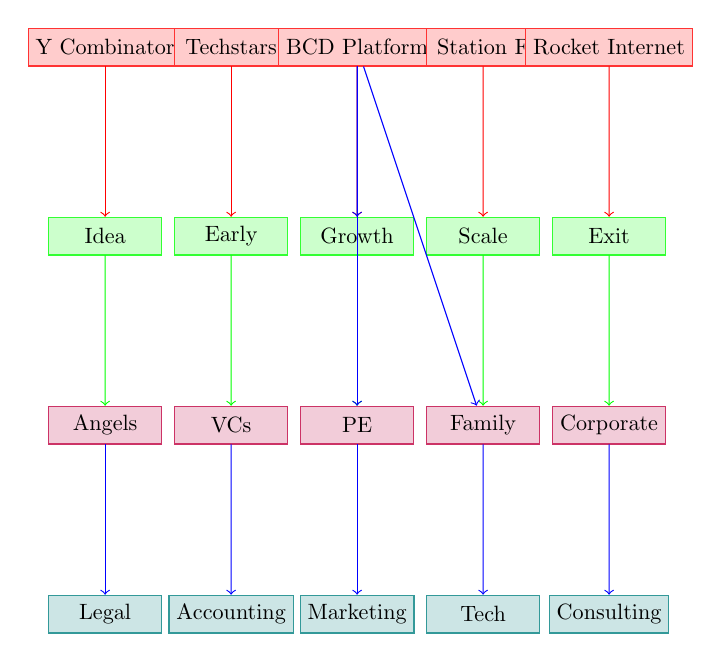
\begin{tikzpicture}[
    scale=0.8,
    transform shape,
    box/.style={rectangle, draw, minimum width=1.8cm, minimum height=0.6cm, align=center},
    ecosystem/.style={box, fill=red!20, draw=red!80},
    startup/.style={box, fill=green!20, draw=green!80},
    investor/.style={box, fill=purple!20, draw=purple!80},
    service/.style={box, fill=teal!20, draw=teal!80},
    arrow/.style={->}
]

% Ecosystem Players
\node[ecosystem] (ycombinator) at (-4,3) {Y Combinator};
\node[ecosystem] (techstars) at (-2,3) {Techstars};
\node[ecosystem] (bcd) at (0,3) {BCD Platform};
\node[ecosystem] (station) at (2,3) {Station F};
\node[ecosystem] (rocket) at (4,3) {Rocket Internet};

% Startup Stages
\node[startup] (idea) at (-4,0) {Idea};
\node[startup] (early) at (-2,0) {Early};
\node[startup] (growth) at (0,0) {Growth};
\node[startup] (scale) at (2,0) {Scale};
\node[startup] (exit) at (4,0) {Exit};

% Investors
\node[investor] (angels) at (-4,-3) {Angels};
\node[investor] (vcs) at (-2,-3) {VCs};
\node[investor] (pe) at (0,-3) {PE};
\node[investor] (family) at (2,-3) {Family};
\node[investor] (corporate) at (4,-3) {Corporate};

% Supporting Services
\node[service] (legal) at (-4,-6) {Legal};
\node[service] (accounting) at (-2,-6) {Accounting};
\node[service] (marketing) at (0,-6) {Marketing};
\node[service] (tech) at (2,-6) {Tech};
\node[service] (consulting) at (4,-6) {Consulting};

% Connections
\draw[arrow, red] (ycombinator) -- (idea);
\draw[arrow, red] (techstars) -- (early);
\draw[arrow, red] (bcd) -- (growth);
\draw[arrow, red] (station) -- (scale);
\draw[arrow, red] (rocket) -- (exit);

\draw[arrow, green] (idea) -- (angels);
\draw[arrow, green] (early) -- (vcs);
\draw[arrow, green] (growth) -- (pe);
\draw[arrow, green] (scale) -- (family);
\draw[arrow, green] (exit) -- (corporate);

\draw[arrow, blue] (angels) -- (legal);
\draw[arrow, blue] (vcs) -- (accounting);
\draw[arrow, blue] (pe) -- (marketing);
\draw[arrow, blue] (family) -- (tech);
\draw[arrow, blue] (corporate) -- (consulting);

% BCD's unique connections
\draw[arrow, blue] (bcd) -- (growth);
\draw[arrow, blue] (bcd) -- (pe);
\draw[arrow, blue] (bcd) -- (family);

\end{tikzpicture}
\caption{Broader Startup Ecosystem Integration}
\label{fig:startup-ecosystem}
\end{figure}

\section{Ecosystem Analysis Insights}

\subsection{Platform Positioning}
BCD occupies a unique position in the business networking ecosystem, bridging the gap between traditional networking platforms and investment-focused communities. The platform's integration with the broader startup ecosystem positions it as a key player in the growth stage of business development.

\subsection{Value Network Analysis}
The ecosystem analysis reveals several key insights:
\begin{itemize}
    \item BCD serves as a critical node connecting entrepreneurs, investors, and service providers
    \item The platform's focus on deal flow creates unique value propositions for all ecosystem participants
    \item Regional focus on DACH provides competitive advantages in local market knowledge
    \item Integration with broader startup ecosystem enables cross-pollination of opportunities
\end{itemize}

\subsection{Competitive Positioning Strategy}
Based on the comprehensive competitor analysis, BCD's strategic positioning should focus on:
\begin{itemize}
    \item \textbf{Regional Expertise:} Leveraging deep DACH market knowledge and local networks
    \item \textbf{Digital-First Approach:} Modern technology platform with seamless user experience
    \item \textbf{Deal Flow Focus:} Specialized focus on quality deal flow and investment opportunities
    \item \textbf{Exclusive Community:} Curated membership with high-quality network connections
    \item \textbf{Cross-Ecosystem Integration:} Strategic partnerships with accelerators, incubators, and service providers
\end{itemize}

\subsection{Market Opportunity Assessment}
The detailed competitor and stakeholder analysis reveals significant market opportunities:
\begin{itemize}
    \item \textbf{Growing Market:} Increasing demand for high-quality business networking platforms
    \item \textbf{Digital Transformation:} Shift towards digital-first networking approaches
    \item \textbf{Regional Gaps:} Opportunities in DACH region for specialized networking platforms
    \item \textbf{Ecosystem Integration:} Growing need for cross-ecosystem collaboration and integration
    \item \textbf{Deal Flow Specialization:} Increasing demand for quality deal flow and investment opportunities
\end{itemize} 